


\section{Einf"uhrung}

\subsection{Beherrschung von Software-Fehlern}

\subsubsection{Arten der Software-Inkorrektheit}


\begin{wrapfigure}{r}{3cm}
    %\fbox{
        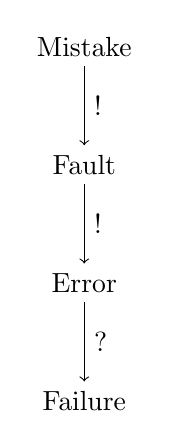
\begin{tikzpicture}

            \node (mistake) at (0,0)    {Mistake};
            \node (fault)   at (0,-1.5)   {Fault};
            \node (error)   at (0,-3)   {Error};
            \node (failure) at (0,-4.5)   {Failure};

            \draw[->] (mistake) -- node[right] {!} (fault);
            \draw[->] (fault) -- node[right] {!} (error);
            \draw[->] (error) -- node[right] {?} (failure);

        \end{tikzpicture}
    %} 
\end{wrapfigure}

\begin{description}
    \item[Irrtum] Modellfehler, Unachtsamkeit, Denkfalle, Unverm"ogen
    \item[(Produkt-) Fehler] Abweichung zwischen Absicht und Realisierung
    \item[Fehlerhafter Zustand] inkorrekter Wert einer internen Variablen
    \item[Versagen] tritt auf, wenn die erbrachte Leistung nicht mehr mit der erw"unschten "ubereinstimmt
\end{description}

\clearpage


\subsubsection{Ma"snahmen zur Fehlerbehersschung}

\begin{description}
    \item[Konstruktive Ma"snahmen zur Irrtumsvermeidung] Kontrolliertes, durchg"angiges, r"uckverfolgbares, transparentes Vorgehen
    \item[Analytische Ma"snahmen zur Fehlererkennung] rigorose, dokumentierte und reproduzierbare Qualit"atssicherung vor Verlassen jeder Prozessphase
    \item[Redundante Ma"snahmen zur Fehlertolerierung] (f"ur hochsicherheitskritische Systeme; au"serhalb des Rahmens dieser Vorlesung)
\end{description}


\subsection{Vorgehensmodelle}

\subsubsection{Prozessmodell}

\begin{itemize}
\item Ein \textbf{Softwareprozess} ist eine Abfolge von Aktivit"aten und daraus resultierenden Erbebnissen, die zur Herstellung eines Softwareprodukts f"uhren.
\item Ein \textbf{Prozessmodell} ist eine vereinfachte (abstrahierte) Beschreibung eines Softwareprozesses und soll insbesondere foltendes festlegen:
    \begin{itemize}
    \item Reihenfolge des Arbeitsablaufes (Entwicklungsstufen, Phasenkonzepte)
    \item Jeweils durchzuf"uhrende Aktivit"aten
    \item Definition der Teilprodukte einschlie"slich Layout und Inhalt
    \item Fertigstellungskriterien (Wann ist ein Teilprodukt fertig gestellt?)
    \item Notwendige Mitarbeiterqualifikationen
    \item Verantwortlichkeiten und Kompetenzen
    \item Anzuwendende Standards, Richtlinien, Methoden und Werkzeuge
    \end{itemize}
\end{itemize}


\subsubsection{Software-Lebenszyklus}

\begin{itemize}
    \item Anforderungsphase
    \item Spezifikationsphase
    \item Entwurfsphase
    \item Implementationspahse
    \item Integrationsphase
    \item Installations-, Nutzungs-, Wartungs-, Abl"osephase
\end{itemize}

\subsubsection{Wasserfall-Modell}
\includegraphics[scale=0.5]{./inc/Einfuehrung/wasserfall.png}

\subsubsection{Das V-Modell}

Erweiterung des Wasserfall-Modells in Hinblick auf die beiden Qualit"atssicherungsaspekte 
\begin{itemize}
    \item Verifikation
    \item Validierung
\end{itemize}

Unter \textbf{Verifikation} wird die "Uberpr"ufung der "Ubereinstimmung zwischen einem Software-Produkt und der Spezifikation verstanden.\\
\textbf{Frage: Are we doing things right?}\\

Unter \textbf{Validierung} wird die "Uberpruefung der Eignung eines Softwareprodukts bezogen auf seinen Einsatzzweck berstanden\\
\textbf{Frage: Are we doing right things?}\\


\includegraphics[scale=0.5]{./inc/Einfuehrung/v-modell.png}


